\documentclass[12pt,a4paper]{article}

% Essential packages
\usepackage[utf8]{inputenc}
\usepackage[english]{babel}
\usepackage{graphicx}
\usepackage{float}
\usepackage{hyperref}
\usepackage{booktabs}
\usepackage{array}
\usepackage{geometry}
\usepackage{amsmath}

% Packages for native diagrams (TikZ)
\usepackage{tikz}
\usetikzlibrary{shapes.geometric, arrows.meta, positioning, fit, backgrounds}

% Margin configuration
\geometry{
    left=2.5cm,
    right=2.5cm,
    top=3cm,
    bottom=3cm
}

% Hyperlink configuration
\hypersetup{
    colorlinks=true,
    linkcolor=blue,
    urlcolor=blue,
    citecolor=black
}

\begin{document}

% ==========================================
% TITLE PAGE
% ==========================================
\begin{titlepage}
    \centering
    \vspace*{1cm}
    
    {\Large \textbf{Universidad Distrital Francisco José de Caldas}} \\
    \vspace{0.5cm}
    {\large School of Engineering \\ Systems Engineering Program} \\
    
    \vspace{3cm}
    
    {\Huge \textbf{Technical Report:}} \\
    \vspace{0.5cm}
    {\Large \textbf{Smart Campus Energy Management System at Sabio Caldas Headquarters: A Systems Analysis and Design Approach}} \\
    
    \vspace{3cm}
    
    \textbf{Authors:} \\
    Omar Yesid Fonseca López (\texttt{oyfonsecal@udistrital.edu.co}) \\
    Daniel Felipe Barrera Suárez (\texttt{dfbarreras@udistrital.edu.co}) \\
    Daniel Mateo Ballesteros Molina (\texttt{dmballesterosm@udistrital.edu.co}) \\
    Dania Lizeth Guzmán Triviño (\texttt{dlguzmant@udistrital.edu.co}) \\
    
    \vfill
    
    \textbf{Course:} Systems Analysis \& Design \\
    \textbf{Professor:} Eng. Carlos Andrés Sierra, M.Sc. \\
    
    \vspace{1cm}
    Bogotá, Colombia \\
    2026
    
\end{titlepage}

% ==========================================
% INDICES AND ABSTRACT
% ==========================================
\pagenumbering{roman}

\begin{abstract}
This report addresses the problem of inefficient energy consumption in the laboratories of the Engineering Faculty, characterized by the prolonged use of computing equipment and lighting systems in unoccupied spaces—a phenomenon strongly influenced by human behavior. Based on a preliminary systems analysis utilizing direct observation, structured surveys, and environmental correlation, we identified patterns of energy waste and institutional limitations, particularly regarding strict IT security policies that restrict the implementation of traditional hardware-based or centralized network solutions. In response to these conditions, this document outlines the design of a decentralized, software-defined solution intended to operate within the user-space. This is achieved through autonomous agents capable of monitoring inactivity, generating deterrent alerts (nudges), and executing energy-saving actions without requiring administrative privileges or modifications to the existing infrastructure.
\end{abstract}

\newpage
\tableofcontents
\newpage
\listoffigures
\newpage

\pagenumbering{arabic}

% ==========================================
% 1. INTRODUCTION
% ==========================================
\section{Introduction}
Efficient energy management in university environments is a critical issue due to the economic and environmental impact of electricity consumption, especially in computer laboratories where equipment and lighting remain active even in the absence of users. In these spaces, human behavior acts as a determining factor in energy waste, creating a gap between institutional sustainability policies and actual practices.

The preliminary analysis identified inefficient usage patterns associated with negligence and lack of awareness, as well as limitations in data collection methods, including survey biases, behavior alteration through observation (Hawthorne effect), and restrictions on directly measuring energy consumption. Although an IoT sensor-based solution might seem appropriate, the institutional context imposes significant constraints, such as the lack of administrative privileges, the prohibition of private perimeter networks, and the inability to deploy additional physical infrastructure.

Given these conditions, this project proposes a software-based approach utilizing autonomous agents that operate within the user-space to monitor equipment activity, generate deterrent alerts, and execute energy-saving actions such as automatic system suspension. This approach addresses the problem without intervening in the existing infrastructure, integrating technical and behavioral aspects into a viable solution adapted to the institutional environment.

% ==========================================
% 2. LITERATURE REVIEW
% ==========================================
\section{Literature Review}
Energy management in higher education institutions has established itself as a relevant field due to its impact on operational efficiency, cost reduction, and environmental sustainability. Several studies agree that university buildings exhibit high levels of energy consumption, particularly in lighting, HVAC, and computing equipment, highlighting stand-by consumption as a significant source of waste \cite{b1, b4}. Furthermore, it is widely recognized that user behavior is a decisive factor in energy inefficiency, introducing a socio-technical dimension to the problem \cite{b3}.

Methodologically, the literature shows a trend towards structured approaches based on energy diagnostics, audits, and the application of frameworks such as the ISO 50001 standard, following continuous improvement cycles (PDCA) and processes for measurement, analysis, and implementation of corrective actions \cite{b2, b4}. These approaches usually rely on direct energy consumption measurements, technical instrumentation, and quantitative data analysis.

However, in university contexts with technical and administrative restrictions—such as the inability to modify infrastructure or measure real power consumption—the need for alternative approaches arises. In this regard, the analyzed project aligns with the literature in its diagnostic phase but differs methodologically by utilizing proxy variables, such as equipment activity and inactivity times, rather than direct energy measurements.

% ==========================================
% 3. OBJECTIVES AND SCOPE
% ==========================================
\section{Objectives and Scope}

\subsection{General Objective}
To design a software-based solution for the efficient management of energy consumption in university laboratories by monitoring computing equipment activity and implementing automatic intervention mechanisms that reduce energy waste without requiring modifications to the institutional infrastructure.

\subsection{Specific Objectives}
\begin{itemize}
    \item To identify patterns of energy usage and waste in laboratories based on the analysis of user behavior and operational environmental conditions.
    \item To analyze the technical and institutional constraints that limit the implementation of traditional solutions based on physical hardware or centralized infrastructure.
    \item To design a distributed monitoring model based on autonomous agents operating within the user-space of each workstation.
    \item To define intervention mechanisms aimed at reducing energy consumption, such as deterrent alerts and automatic suspension of idle equipment.
\end{itemize}

\subsection{Scope}
The scope of this project encompasses the design and implementation of a solution aimed at efficient energy consumption management in university environments, specifically in the laboratories of the Engineering Faculty. The project's development is initially planned as a focused, small-scale pilot (Proof of Concept - PoC), implemented on a limited set of workstations within a specific laboratory. This approach allows for the evaluation of the technical and operational viability of the solution under controlled conditions before potential institutional scalability.

% ==========================================
% 4. ASSUMPTIONS AND LIMITATIONS
% ==========================================
\section{Assumptions and Limitations}

\subsection{Assumptions}
For the proper development and design of the Proof of Concept (PoC), the following operational assumptions were established:
\begin{itemize}
    \item \textbf{Network Stability:} It is assumed that the laboratory workstations have a stable perimeter connection (Wi-Fi or Ethernet) that allows outbound HTTPS requests for transmitting logs to the cloud database and the messaging API.
    \item \textbf{Computational Load:} It is assumed that a processor (CPU) load of less than 20\% is a reliable technical indicator that the equipment is not executing critical background tasks (e.g., 3D rendering or heavy simulations).
    \item \textbf{Execution Permissions:} It is presumed that, although users do not possess administrator privileges, local Windows policies permit the execution of standalone scripts (\textit{.exe}) from the \textit{Startup} folder and the calling of power state libraries (\textit{powrprof.dll}) to suspend the machine.
\end{itemize}

\subsection{Limitations}
The development of this project is conditioned by technical and institutional constraints. The inability to obtain administrative privileges restricts software installation at the system level (e.g., Windows services or Active Directory GPOs). Similarly, security policies prohibit the use of internal central servers, which forced the architecture toward a decentralized approach.

Additionally, due to electrical safety restrictions, it is not possible to deploy physical sensors or access real consumption data in kilowatts (kWh). Consequently, the project relies on proxy variables (peripheral inactivity time), meaning that the energy-saving results will be indirect mathematical estimations.

% ==========================================
% 5. METHODOLOGY AND SOLUTION DESIGN
% ==========================================
\section{Methodology and Solution Design}
The methodology is structured in phases of systems analysis applied to a socio-technical problem.

\subsection{Phases 1 and 2: Systems Analysis and Feasibility}
Complementary sources such as illuminance measurement, habit surveys (n=35), and direct observation were utilized. The results showed that the main factor of waste is associated with human forgetfulness. When analyzing feasibility, traditional IoT solutions were discarded due to infrastructure roadblocks, redefining the project toward a Software-Defined environment.

\subsection{Phase 3: Architecture Design}
A distributed system operating via autonomous agents was designed. As observed in Figure \ref{fig:arch}, the agent runs in the User-Space without requiring administrative installation. It communicates with the operating system APIs to gather telemetry and sends its states to a cloud database (MySQL DBaaS) and notifications to an external messaging API.

\begin{figure}[H]
\centering
\resizebox{0.85\textwidth}{!}{%
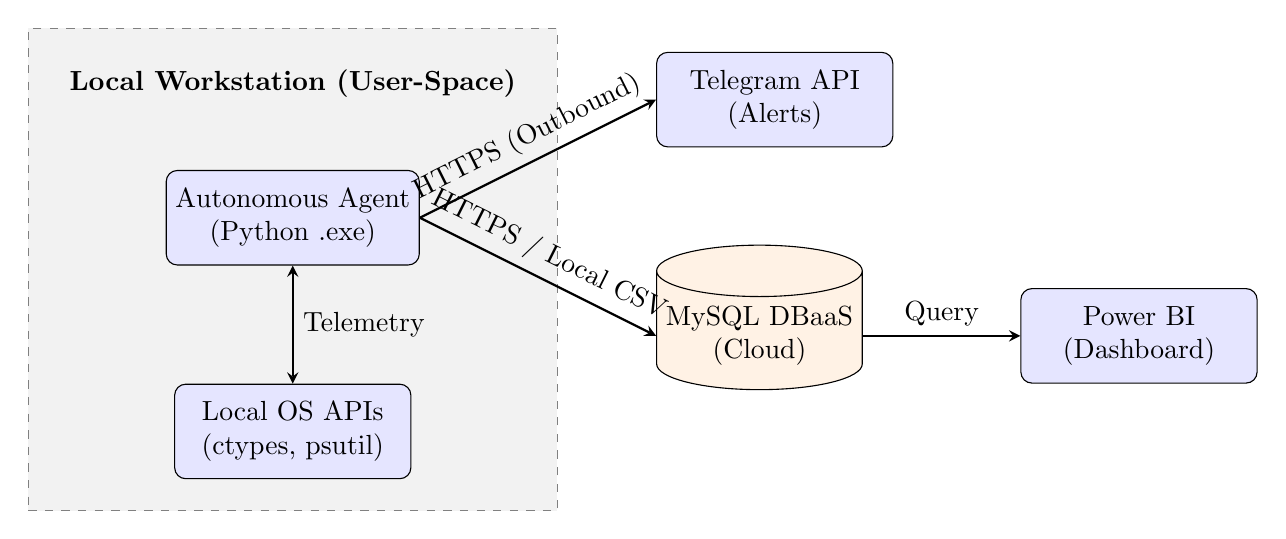
\begin{tikzpicture}[
    node distance=2cm and 3cm,
    box/.style={draw, rectangle, minimum width=3cm, minimum height=1.2cm, align=center, fill=blue!10, rounded corners},
    db/.style={draw, cylinder, shape border rotate=90, aspect=0.25, minimum height=1.5cm, minimum width=2.2cm, align=center, fill=orange!10},
    arrow/.style={->, >=stealth, thick}
]

\node[box] (agent) {Autonomous Agent \\ (Python .exe)};
\node[box, below=1.5cm of agent] (os) {Local OS APIs \\ (ctypes, psutil)};

\node[above=0.8cm of agent] (title) {\textbf{Local Workstation (User-Space)}};

\begin{scope}[on background layer]
    \node[fill=gray!10, draw=gray, dashed, fit=(title) (agent) (os), inner sep=0.4cm] (pc) {};
\end{scope}


\node[box, right=3cm of agent, yshift=1.5cm] (telegram) {Telegram API \\ (Alerts)};
\node[db, right=3cm of agent, yshift=-1.5cm] (mysql) {MySQL DBaaS \\ (Cloud)};
\node[box, right=2cm of mysql] (powerbi) {Power BI \\ (Dashboard)};

\draw[arrow, <->] (agent) -- node[right] {Telemetry} (os);
\draw[arrow] (agent.east) -- node[above, sloped] {HTTPS (Outbound)} (telegram.west);
\draw[arrow] (agent.east) -- node[above, sloped] {HTTPS / Local CSV} (mysql.west);
\draw[arrow] (mysql.east) -- node[above] {Query} (powerbi.west);

\end{tikzpicture}%
}
\caption{Decentralized Software-Defined System Architecture}
\label{fig:arch}
\end{figure}

\section{Implementation, Expected Results, and Discussion}

\subsection{Operational Implementation Logic}
The autonomous agent implements a multi-stage intervention logic to guarantee the safety of user data. As illustrated in the flowchart (Figure \ref{fig:flow}), the system continuously verifies peripheral inactivity. If it exceeds 15 minutes, it introduces a complexity layer by checking the CPU load. Only if the machine is genuinely idle is a deterrent visual alert ("Nudge") launched. If the user does not cancel this alert, the system proceeds with a safe OS Suspend.

\begin{figure}[H]
\centering
\resizebox{0.75\textwidth}{!}{%
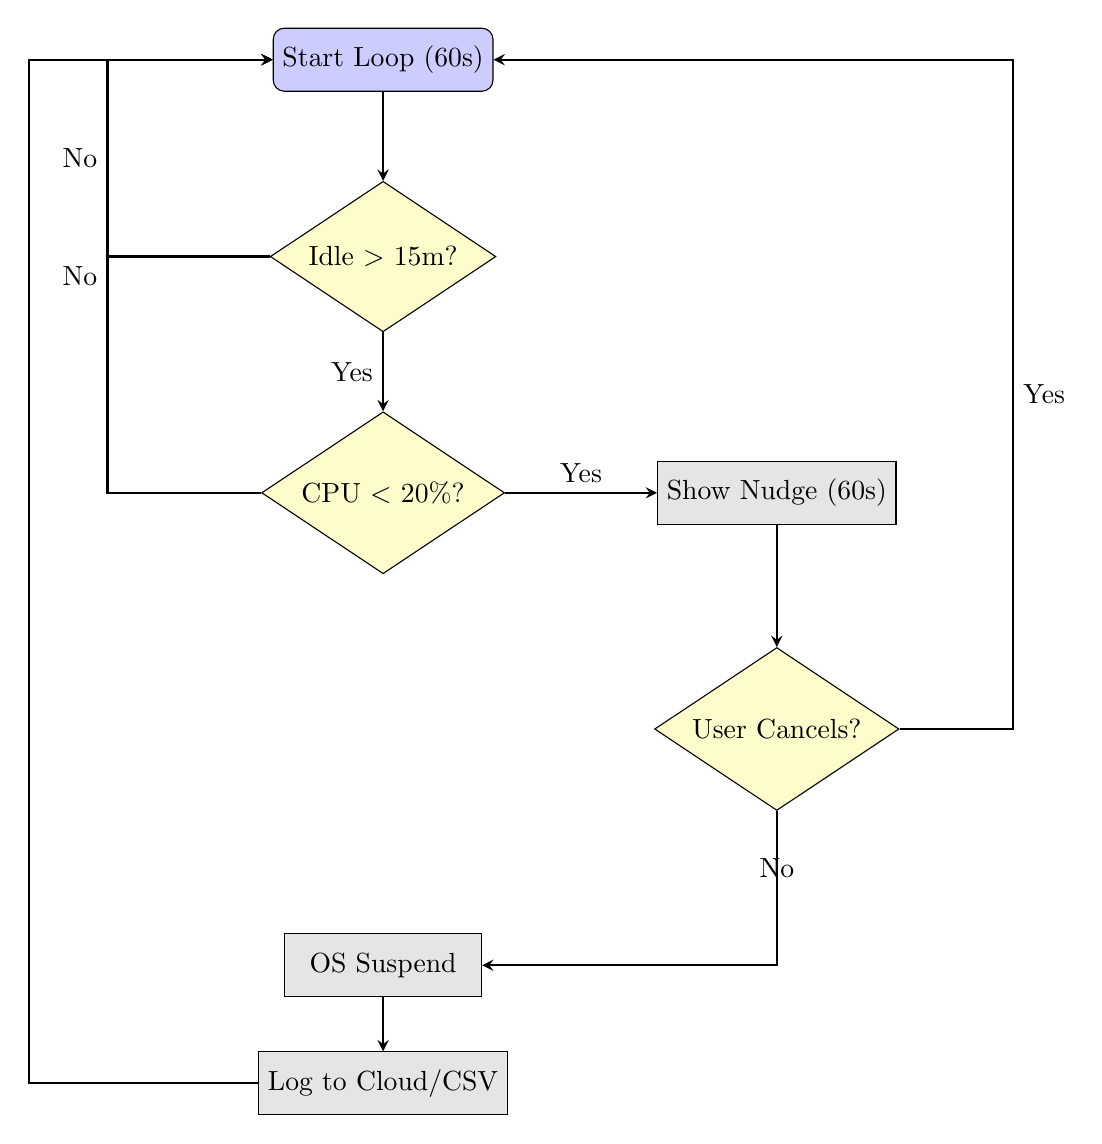
\begin{tikzpicture}[
    node distance=1.5cm,
    startstop/.style={rectangle, rounded corners, minimum width=2.5cm, minimum height=0.8cm, text centered, draw=black, fill=blue!20},
    process/.style={rectangle, minimum width=2.5cm, minimum height=0.8cm, text centered, draw=black, fill=gray!20},
    decision/.style={diamond, minimum width=2.5cm, minimum height=0.8cm, text centered, draw=black, fill=yellow!20, aspect=1.5},
    arrow/.style={thick,->,>=stealth}
]

% Nodos
\node (start) [startstop] {Start Loop (60s)};
\node (idle) [decision, below of=start, yshift=-1cm] {Idle $>$ 15m?};
\node (cpu) [decision, below of=idle, yshift=-1.5cm] {CPU $<$ 20\%?};
\node (nudge) [process, right of=cpu, xshift=3.5cm] {Show Nudge (60s)};
\node (cancel) [decision, below of=nudge, yshift=-1.5cm] {User Cancels?};
\node (suspend) [process, below of=cpu, yshift=-4.5cm] {OS Suspend};
\node (log) [process, below of=suspend] {Log to Cloud/CSV};

% Flechas
\draw [arrow] (start) -- (idle);
\draw [arrow] (idle) -- node[anchor=east] {Yes} (cpu);
\draw [arrow] (idle) -- ++(-3.5,0) |- node[anchor=east, near start] {No} (start);
\draw [arrow] (cpu) -- node[anchor=south] {Yes} (nudge);
\draw [arrow] (cpu) -- ++(-3.5,0) |- node[anchor=east, near start] {No} (start);
\draw [arrow] (nudge) -- (cancel);
\draw [arrow] (cancel) -- ++(3,0) |- node[anchor=west, near start] {Yes} (start);
\draw [arrow] (cancel) |- node[anchor=south, near start] {No} (suspend);
\draw [arrow] (suspend) -- (log);
\draw [arrow] (log) -- ++(-4.5,0) |- (start);

\end{tikzpicture}%
}
\caption{Agent Operational Workflow and Decision Logic}
\label{fig:flow}
\end{figure}

\subsection{Expected Results and Discussion}
The system's implementation is expected to achieve a measurable reduction in the idle time of powered-on equipment, directly combating the human factor bias. Automating suspension based on nudges and inactivity will mitigate negligence without requiring investment in physical IT infrastructure.

The proposal introduces a paradigm shift: compared to solutions demanding physical sensors or electrical panel modifications, control from the User-Space is infinitely more scalable and economical, serving as a replicable model for public institutions with constrained resources and locked infrastructures.

\section{Conclusions}
This work addressed the problem of inefficient energy consumption from a socio-technical perspective, highlighting that energy waste primarily originates from human behavioral dynamics. Institutional restrictions led to rethinking the problem towards a decentralized, software-defined solution, demonstrating that it is possible to manage resource usage by shifting intelligence from physical infrastructure to the logical layer of the operating system.

Although this project operates as a Proof of Concept, the developed design establishes a solid, scalable conceptual foundation that respects cybersecurity policies, opening the possibility for massive deployments that facilitate the university's transition towards a "Smart Campus".


\newpage
\begin{thebibliography}{9}

\bibitem{b1} M. V. Doblari, \textit{Gestión integral de energía en instituciones universitarias. Caso: Edificio Eva Duarte de Perón UNNOBA}, Master's Thesis, Universidad Nacional del Noroeste de la Provincia de Buenos Aires, Argentina, n.d.

\bibitem{b2} M. Abad Mier, \textit{Gestión energética de la biblioteca universitaria de la UVA, aplicando la ISO 50001}, Bachelor's Thesis, Universidad de Valladolid, Spain, 2015.

\bibitem{b3} J. C. Figueroa Sandrez, ``Gestión energética sostenible y su impacto en la huella de carbono: estudio de caso universitario,'' \textit{Journal of Management \& Business Studies}, vol. 7, 2025.

\bibitem{b4} B. Meza-Alcívar, M. Alemán-García, and M. Herrera-Suárez, ``Implementación de un sistema de gestión energético para institutos de educación superior,'' \textit{Revista Científica INGENIAR}, vol. 6, no. 12, 2023.

\bibitem{b5} O. Y. Fonseca López, D. F. Barrera Suárez, D. M. Ballesteros Molina, and D. L. Guzmán Triviño, ``Smart Campus Energy Management System,'' academic presentation, Universidad Distrital Francisco José de Caldas, Colombia, 2026.

\end{thebibliography}

\end{document}